\begin{dang}{Toán thực tế, liên môn liên quan đến giới hạn dãy số}
	$$S=u_1+u_1q+u_1q^2+...=\dfrac{u_1}{1-q}.$$
\end{dang}
\subsubsection*{Ví dụ mẫu}
\begin{vd}%[1C3K1-6]
	\immini{Từ hình vuông có độ dài cạnh bằng $1$, người ta nối các trung điểm của cạnh hình vuông để tạo ra hình vuông mới như hình bên. Tiếp tục quá trình này đến vô hạn.
		\begin{enumEX}{1}
			\item Tính diện tích $S_n$ của hình vuông được tạo thành từ bước thứ $n$.
			\item Tính tổng diện tích của tất cả các hình vuông được tạo thành.
	\end{enumEX}}	
	{
		\begin{tikzpicture}[scale=0.6, font=\footnotesize,>=stealth]
			\def\canhAD{6};
			\coordinate (D) at (0,0);
			\coordinate (A) at ($(D)+(90:\canhAD)$);
			\coordinate (C) at ($(D)+(0:\canhAD)$);
			\coordinate (B) at ($(A)+(0:\canhAD)$);
			\coordinate (E) at ($(A)!0.5!(B)$);
			\coordinate (F) at ($(B)!0.5!(C)$);
			\coordinate (G) at ($(C)!0.5!(D)$);
			\coordinate (H) at ($(D)!0.5!(A)$);
			\coordinate (K) at ($(E)!0.5!(F)$);
			\coordinate (L) at ($(F)!0.5!(G)$);
			\coordinate (M) at ($(G)!0.5!(H)$);
			\coordinate (J) at ($(H)!0.5!(E)$);
			\coordinate (I) at ($(E)!0.5!(G)$);
			\coordinate (X) at ($(J)!0.5!(K)$);
			\coordinate (Y) at ($(K)!0.5!(L)$);
			\coordinate (T) at ($(L)!0.5!(M)$);
			\coordinate (Q) at ($(M)!0.5!(J)$);
			\draw(A) rectangle (C)(E)--(F)--(G)--(H)--cycle (J)--(K)--(L)--(M)--cycle (X)--(Y)--(T)--(Q)--cycle;
			\draw [>=stealth,|<->|] ([shift=({0,-0.4})]D)--([shift=({0,-0.4})]C) node [midway,below]{$1$};
			
			%			\foreach \x/\y in {A/90,D/-90,C/-90,B/90,E/90,G/-90,H/180,F/0,K/90,L/-90,M/-90,J/90,I/-110}{\fill (\x) circle(1pt) ($(\x)+(\y:0.3cm)$) node{$\x$};}
		\end{tikzpicture}
	}
	
	\loigiai{
		\begin{enumerate}
			\item Từ giả thiết suy ra diện tích hình vuông sau bằng $\dfrac{1}{2}$ diện tích hình vuông trước.\\ 
			Khi đó diện tích của các hình vuông tạo thành một cấp số nhân lùi vô hạn với số hạng đầu $S_1=1$ và công bội $q=\dfrac{1}{2}$.\\
			Diện tích $S_n$ của hình vuông được tạo thành từ bước thứ $n$ là $S_n=S_1\cdot q^{n-1}=\left(\dfrac{1}{2}\right)^{n-1}$.
			\item Tổng diện tích của tất cả các hình vuông được tạo thành là:\\
			$$S=\dfrac{u_1}{1-q}=\dfrac{1}{1-\dfrac{1}{2}}=2.$$
		\end{enumerate}
	}
\end{vd}
\begin{vd}%[1C3K1-6]
	Có $1$ kg chất phóng xạ độc hại. Biết rằng, cứ sau một khoảng thời gian $T=24000$ năm thì một nửa số chất phóng xạ này bị phân rã thành chất khác không độc hại đối với sức khỏe của con người ($T$ được gọi là \textit{chu kì bán rã}).
	\begin{flushright}
		(\textit{Nguồn: Đại số và giải tích 11, NXB GD Việt Nam, 2021})
	\end{flushright}
	Gọi $u_n$ là khối lượng chất phóng xạ còn lại sau chu kì thứ $n$.
	\begin{enumerate}
		\item  Tìm số hạng tổng quát $u_n$ của dãy số $(u_n)$.
		\item  Chứng minh rằng $(u_n)$ có giới hạn là $0$.
		\item  Từ kết quả câu $2$, chứng tỏ rằng sau một số năm nào đó khối lượng phóng xạ đã cho ban đầu không còn độc hại với con người, biết rằng chất phóng xạ này sẽ không độc hại nữa nếu khối lượng chất phóng xạ còn lại bé hơn $10^{-6}$ g.
	\end{enumerate}
	\loigiai{
		\begin{enumerate}
			\item  Khối lượng chất phóng xạ còn lại sau chu kì bán rã thứ $1$ là $u_1=\dfrac{1}{2}\cdot 1=1$ kg.\\
			Khối lượng chất phóng xạ còn lại sau chu kì bán rã thứ $2$ là $u_2=\dfrac{1}{2}\cdot u_1=\dfrac{1}{2}\cdot \dfrac{1}{2}=\dfrac{1}{2^2}$ kg.\\
			Khối lượng chất phóng xạ còn lại sau chu kì bán rã thứ $3$ là $u_3=\dfrac{1}{2}\cdot u_2=\dfrac{1}{2}\cdot \dfrac{1}{4}=\dfrac{1}{2^3}$ kg.\\
			Khối lượng chất phóng xạ còn lại sau chu kì bán rã thứ $n$ là $u_n=\dfrac{1}{2^n}$ kg.\\
			\item $\lim \limits_{n \to +\infty}u_n=\lim \limits_{n \to +\infty}\dfrac{1}{2^n}=\lim\left(\dfrac{1}{2}\right)^n=0$.
			\item Chất phóng xạ sẽ không độc hại nữa nếu khối lượng chất phóng xạ còn lại bé hơn $10^{-6}~\mathrm{g}=10^{-9}$ kg
			$$\Leftrightarrow u_n<10^{-9}\Leftrightarrow\dfrac{1}{2^n}<10^{-9}\Leftrightarrow 2^n>10^9\Leftrightarrow n\geq 30.$$
			Vậy sau ít nhất $30$ chu kì bằng $30\cdot 24000=720000$ năm thì khối lượng phóng xạ đã cho ban đầu không còn độc hại với con người nữa.
		\end{enumerate}
	}
\end{vd}
\begin{vd}%[1C3G1-6]
	Gọi $C$ là nữa đường tròn đường kính $AB=2R$.\\
	$C_1$ là đường gồm hai nửa đường tròn đường kính $\dfrac{AB}{2}$,\\
	$C_2$ là đường gồm bốn nửa đường tròn đường kính $\dfrac{AB}{4},\cdots$\\
	$C_n$ là đường gồm $2^n$ nửa đường tròn đường kính $\dfrac{AB}{2^n},\cdots$
	\immini{	Gọi $p_n$ là độ dài của $C_n$, $S_n$ là diện tích hình phẳng giới hạn bởi $C_n$ và đoạn thẳng $AB$.
		\begin{enumEX}{1}
			\item Tính $p_n$, $S_n$.
			\item Tính giới hạn của các dãy số $(p_n)$ và $(S_n)$.
		\end{enumEX}
	}{
		\begin{tikzpicture}[declare function={r=3;}]
			\path
			(0,0) coordinate (O)
			(0:r) coordinate (A)
			(180:r) coordinate (B)
			($(A)!.5!(O)$) coordinate (M)
			($(B)!.5!(O)$) coordinate (N)
			($(B)!.5!(N)$) coordinate (I)
			($(N)!.5!(O)$) coordinate (J)
			($(O)!.5!(M)$) coordinate (K)
			($(M)!.5!(A)$) coordinate (H)
			($(B)!.5!(I)$) coordinate (Q);
			\draw (A) arc(0:180:r) (A) arc(0:180:r/2) (O) arc(0:180:r/2) (A) arc(0:180:r/4) (A) arc(0:180:r/4)(M) arc(0:180:r/4) (O) arc(0:180:r/4) (N) arc(0:180:r/4)
			(A) arc(0:180:r/8) (H) arc(0:180:r/8) (M) arc(0:180:r/8) (K) arc(0:180:r/8) (O) arc(0:180:r/8) (J) arc(0:180:r/8) (N) arc(0:180:r/8) (I) arc(0:180:r/8);
			\draw (A)--(B);
			\path 
			($(O)+(90:0.9*r)$) node{$C$}
			($(N)+(90:0.4*r)$) node[scale=0.8]{$C_1$}
			($(I)+(90:0.18*r)$) node[scale=0.7]{$C_2$}
			($(Q)+(90:0.06*r)$) node[scale=0.6]{$C_3$};
			\foreach \x/\y in {A/-90, B/-90}{\fill (\x) circle(1pt) ($(\x)+(\y:0.3cm)$) node{$\x$};}
		\end{tikzpicture}
	}
	
	\loigiai{
		\begin{enumerate}
			\item Ta có  
			\begin{eqnarray*}
				p_n&=&2^n \cdot \pi r=2^n\cdot\pi \cdot \dfrac{AB}{2\cdot2^n}\\
				&=&\dfrac{\pi AB}{2}\\
				&=&\dfrac{\pi \cdot 2R}{2}\\
				&=&\pi R.
			\end{eqnarray*}
			\begin{eqnarray*}
				S_n&=&2^n \cdot \dfrac{1}{2}\pi r^2\\
				&=&2^n \cdot \dfrac{1}{2}\pi \left(\dfrac{AB}{2\cdot2^n}\right)^2\\
				&=&2^n \cdot \dfrac{1}{2}\pi \left(\dfrac{2R}{2\cdot2^n}\right)^2\\
				&=&2^n \cdot \dfrac{1}{2}\pi \dfrac{R^2}{(2^n)^2}\\
				&=&\dfrac{\pi R^2}{2^{n+1}}.	
			\end{eqnarray*}			
			\item $\lim \limits_{n \to +\infty}p_n=\lim \limits_{n \to +\infty}\left(\pi R\right) = \pi R$.\\
			$\lim \limits_{n \to +\infty}S_n=\lim \limits_{n \to +\infty}\dfrac{\pi R^2}{2^{n+1}}=0$ (Vì $\lim \limits_{n \to +\infty}\left(\pi R^2\right)=\pi R^2$ và $\lim \limits_{n \to +\infty}2^{n+1}=+\infty$).
		\end{enumerate}
	}
\end{vd}
\begin{vd}%[1D4K1-6]
	\immini{Từ độ cao $55,8 \mathrm{~m}$ của tháp nghiêng Pisa nước Ý, người ta thả một quả bóng cao su chạm xuống đất hình bên dưới. Giả sử mỗi lần chạm đất quả bóng lại nảy lên độ cao bằng $\dfrac{1}{10}$ độ cao mà quả bóng đạt được trước đó. Gọi $S_n$ là tổng độ dài quãng đường di chuyển của quả bóng tính từ lúc thả ban đầu cho đến khi quả bóng đó chạm đất $n$ lần. Tính $\lim \limits_{n \to +\infty}S_n$.}{
		
		\definecolor{lightcornflowerblue}{rgb}{0.6, 0.81, 0.93}
		\definecolor{cadmiumgreen}{rgb}{0.0, 0.42, 0.24}
		\definecolor{trueblue}{rgb}{0.0, 0.45, 0.81}
		\definecolor{tumbleweed}{rgb}{0.87, 0.67, 0.53}%màu cát
		\begin{tikzpicture}[line join=round, line cap=round,scale=1,transform shape]
			\clip (-4,-3.5) rectangle (4,3.5);
			\tikzset{thap/.pic={%Xây từ dưới lên
					\def\T{ 
						(-.88,-1.78)%1
						..controls +(40:.17) and +(120:.1) ..  (.686,-1.91)--(.68,-1.94)
						..controls +(120:.1) and +(40:.12) ..  (-.87,-1.81)
						--cycle
						
						(-.8,-1.2)%2
						..controls +(40:.14) and +(120:.14) ..  (.72,-1.34)--(.7,-1.36)
						..controls +(120:.1) and +(40:.12) ..  (-.78,-1.23)
						--cycle
						
						(-.74,-.65)%3
						..controls +(40:.22) and +(120:.17) ..  (.74,-.78)--(.72,-.8)
						..controls +(120:.15) and +(40:.15) ..  (-.72,-.67)
						--cycle
						
						(-.68,-.13)%4
						..controls +(40:.34) and +(110:.2) ..  (.8,-.26)--(.78,-.28)
						..controls +(110:.17) and +(40:.27) ..  (-.66,-.15)
						--cycle
						
						(-.65,.36)%5
						..controls +(40:.44) and +(120:.3) ..  (.85,.24)--(.83,.22)
						..controls +(130:.35) and +(40:.35) ..  (-.63,.34)
						--cycle
						
						(-.58,.88)%6
						..controls +(40:.44) and +(120:.3) ..  (.87,.78)--(.85,.76)
						..controls +(130:.35) and +(40:.35) ..  (-.56,.86)
						--cycle
						
						(-.52,1.35)%7
						..controls +(120:.32) and +(110:.47) ..  (.93,1.26)--(.9,1.25)
						..controls +(110:.43) and +(110:.27) ..  (-.49,1.35)
						--cycle
						
						(-.31,2)%8
						..controls +(120:.47) and +(55:.46) ..  (.76,1.94)--(.74,1.94)
						..controls +(75:.31) and +(115:.28) ..  (-.28,2)
						--cycle
						
						(-.48,1.5)
						..controls +(40:.33) and +(110:.2) ..  (.86,1.4)
						(-.476,1.52)
						..controls +(40:.33) and +(110:.2) ..  (.86,1.42)
						(-.472,1.54)
						..controls +(40:.33) and +(110:.2) ..  (.86,1.44)
						(-.468,1.56)
						..controls +(40:.33) and +(110:.2) ..  (.86,1.46)
						
						(-.28,2.2)
						..controls +(40:.27) and +(140:.2) ..  (.74,2.16)
						(-.276,2.22)
						..controls +(40:.27) and +(140:.2) ..  (.74,2.18)
						(-.272,2.24)
						..controls +(40:.27) and +(140:.2) ..  (.74,2.2)
						(-.268,2.26)
						..controls +(40:.27) and +(140:.2) ..  (.74,2.22)
						;}
					\draw \T;
					%\fill[tumbleweed] \T;
			}}
			
			\tikzset{rao/.pic={%Rào
					\def\R{ 
						(-.48,1.5)
						..controls +(40:.33) and +(110:.2) ..  (.86,1.4)
						(-.476,1.52)
						..controls +(40:.33) and +(110:.2) ..  (.86,1.42)
						(-.472,1.54)
						..controls +(40:.33) and +(110:.2) ..  (.86,1.44)
						(-.468,1.56)
						..controls +(40:.33) and +(110:.2) ..  (.86,1.46)
						
						(-.28,2.2)
						..controls +(40:.27) and +(140:.2) ..  (.74,2.16)
						(-.276,2.22)
						..controls +(40:.27) and +(140:.2) ..  (.74,2.18)
						(-.272,2.24)
						..controls +(40:.27) and +(140:.2) ..  (.74,2.2)
						(-.268,2.26)
						..controls +(40:.27) and +(140:.2) ..  (.74,2.22)
						;}
					\draw \R;
					%\fill[tumbleweed] \R;
			}}
			
			\tikzset{co/.pic={%Cờ
					\def\C{ 
						(0.1,2.3)--(.1,2.9)
						(.1,2.82)
						..controls +(-40:.2) and +(140:.22) ..  (.2,2.6)
						..controls +(-60:0) and +(100:.1) ..(.16,2.5)
						..controls +(140:.1) and +(-30:0) ..  (.1,2.53)--cycle
						;}
					\draw \C;
					\fill[red] \C;
			}}
			
			\tikzset{cong0/.pic={%Đường cong trệt
					\def\D0{ 
						(.68,-1.96)
						..controls +(120:.1) and +(40:.12) ..  (-.87,-1.81)--
						(-.87,-1.94)
						..controls +(80:.12) and +(95:0.12) ..  (-.68,-2.06)
						..controls +(80:.12) and +(85:0.3) ..  (-.4,-2.12)
						..controls +(80:.25) and +(95:0.25) ..  (-.02,-2.12)
						..controls +(80:.25) and +(95:0.25) ..  (.27,-2.14)
						..controls +(80:.12) and +(95:0.12) ..  (.5,-2.14)
						..controls +(70:.12) and +(95:0.02) ..  (.66,-2.1)--cycle
						;}
					\draw \D0;
					\fill[tumbleweed] \D0;
			}}
			
			\tikzset{cong1/.pic={%Đường cong 1
					\def\D1{ 
						(.7,-1.36)
						..controls +(120:.1) and +(40:.12) ..  (-.78,-1.23)--
						(-.78,-1.35)
						..controls +(80:.12) and +(95:0.12) ..  (-.72,-1.35)
						..controls +(80:.12) and +(95:0.12) ..  (-.64,-1.35)
						..controls +(80:.12) and +(95:0.12) ..  (-.55,-1.35)
						..controls +(80:.12) and +(95:0.12) ..  (-.44,-1.36)
						..controls +(80:.12) and +(95:0.12) ..  (-.3,-1.37)
						..controls +(80:.12) and +(95:0.12) ..  (-.14,-1.38)
						..controls +(80:.12) and +(95:0.12) ..  (0.02,-1.39)
						..controls +(80:.12) and +(95:0.12) ..  (0.18,-1.4)
						..controls +(80:.12) and +(95:0.12) ..  (0.32,-1.42)
						..controls +(70:.12) and +(95:0.12) ..  (0.42,-1.44)
						..controls +(70:.12) and +(95:0.12) ..  (0.52,-1.46)
						..controls +(70:.12) and +(95:0.12) ..  (0.6,-1.47)
						..controls +(70:.12) and +(95:0.12) ..  (0.68,-1.5)--cycle
						;}
					\draw \D1;
					\fill[tumbleweed] \D1;
			}}
			
			\tikzset{cong2/.pic={%Đường cong 2
					\def\D2{ 
						(.72,-.8)
						..controls +(120:.15) and +(40:.15) ..  (-.72,-.67)--
						(-.72,-.79)
						..controls +(80:.12) and +(95:0.12) ..  (-.66,-.79)
						..controls +(80:.12) and +(95:0.12) ..  (-.58,-.79)
						..controls +(80:.12) and +(95:0.12) ..  (-.48,-.79)
						..controls +(80:.12) and +(95:0.12) ..  (-.38,-.8)
						..controls +(80:.12) and +(95:0.12) ..  (-.23,-.8)
						..controls +(80:.12) and +(95:0.12) ..  (-0.08,-.81)
						..controls +(80:.12) and +(95:0.12) ..  (0.08,-.82)
						..controls +(80:.12) and +(95:0.12) ..  (0.22,-.84)
						..controls +(80:.12) and +(95:0.12) ..  (0.36,-.85)
						..controls +(70:.12) and +(95:0.12) ..  (0.48,-.87)
						..controls +(70:.12) and +(95:0.12) ..  (0.58,-.89)
						..controls +(70:.12) and +(95:0.12) ..  (0.66,-.9)
						..controls +(70:.12) and +(95:0.12) ..  (0.71,-.92)--cycle
						;}
					\draw \D2;
					\fill[tumbleweed] \D2;
			}}
			
			\tikzset{cong3/.pic={%Đường cong 3
					\def\D3{ 
						(.78,-.28)
						..controls +(110:.17) and +(40:.27) ..  (-.66,-.15)--
						(-.66,-.26)
						..controls +(80:.12) and +(95:0.12) ..  (-.6,-.25)
						..controls +(80:.12) and +(95:0.12) ..  (-.52,-.24)
						..controls +(80:.12) and +(95:0.12) ..  (-.44,-.23)
						..controls +(80:.12) and +(95:0.12) ..  (-.32,-.23)
						..controls +(80:.12) and +(95:0.12) ..  (-.18,-.23)
						..controls +(80:.12) and +(95:0.12) ..  (-.04,-.24)
						..controls +(80:.12) and +(95:0.12) ..  (0.13,-.25)
						..controls +(80:.12) and +(95:0.12) ..  (0.26,-.26)
						..controls +(70:.12) and +(95:0.12) ..  (0.42,-.29)
						..controls +(70:.12) and +(95:0.12) ..  (0.54,-.31)
						..controls +(70:.12) and +(95:0.12) ..  (0.63,-.33)
						..controls +(70:.12) and +(95:0.12) ..  (0.7,-.35)
						..controls +(70:.12) and +(95:0.12) ..  (0.765,-.38)--cycle
						;}
					\draw \D3;
					\fill[tumbleweed] \D3;
			}}
			
			\tikzset{cong4/.pic={%Đường cong 4
					\def\D4{ 
						(.83,.22)
						..controls +(130:.35) and +(40:.35) ..  (-.63,.34)--
						(-.63,.23)
						..controls +(80:.12) and +(95:0.12) ..  (-.57,.25)
						..controls +(80:.12) and +(95:0.12) ..  (-.49,.26)
						..controls +(80:.12) and +(95:0.12) ..  (-.4,.28)
						..controls +(80:.12) and +(95:0.12) ..  (-.27,.3)
						..controls +(80:.12) and +(95:0.12) ..  (-.15,.3)
						..controls +(80:.12) and +(95:0.12) ..  (0.02,.3)
						..controls +(80:.12) and +(95:0.12) ..  (0.16,.29)
						..controls +(80:.12) and +(95:0.12) ..  (0.31,.27)
						..controls +(70:.12) and +(95:0.12) ..  (0.45,.25)
						..controls +(70:.12) and +(95:0.12) ..  (0.58,.23)
						..controls +(70:.12) and +(95:0.12) ..  (0.67,.2)
						..controls +(70:.12) and +(95:0.12) ..  (0.75,.17)
						..controls +(70:.12) and +(95:0.12) ..  (0.8,.14)--cycle
						;}
					\draw \D4;
					\fill[tumbleweed] \D4;
			}}
			
			\tikzset{cong5/.pic={%Đường cong 5
					\def\D5{ 
						(.85,.76)
						..controls +(130:.35) and +(40:.35) ..  (-.56,.86)--
						(-.56,.74)
						..controls +(80:.12) and +(95:0.12) ..  (-.5,.77)
						..controls +(80:.12) and +(95:0.12) ..  (-.44,.79)
						..controls +(80:.12) and +(95:0.12) ..  (-.34,.81)
						..controls +(80:.12) and +(95:0.12) ..  (-.22,.83)
						..controls +(80:.12) and +(95:0.12) ..  (-0.08,.85)
						..controls +(80:.12) and +(95:0.12) ..  (0.06,.85)
						..controls +(80:.12) and +(95:0.12) ..  (0.22,.83)
						..controls +(70:.12) and +(95:0.12) ..  (0.36,.81)
						..controls +(70:.12) and +(95:0.12) ..  (0.5,.78)
						..controls +(70:.12) and +(95:0.12) ..  (0.62,.74)
						..controls +(70:.12) and +(95:0.12) ..  (0.73,.72)
						..controls +(70:.12) and +(95:0.12) ..  (0.82,.68)--cycle
						;}
					\draw \D5;
					\fill[tumbleweed] \D5;
			}}
			
			\tikzset{cong6/.pic={%Đường cong 6
					\def\D6{ 
						(.9,1.25)
						..controls +(110:.43) and +(110:.27) ..  (-.49,1.35)--
						(-.49,1.3)
						..controls +(80:.12) and +(95:0.12) ..  (-.45,1.33)
						..controls +(80:.12) and +(95:0.12) ..  (-.38,1.33)
						..controls +(80:.12) and +(95:0.12) ..  (-.28,1.35)
						..controls +(80:.12) and +(95:0.12) ..  (-.16,1.37)
						..controls +(80:.12) and +(95:0.12) ..  (-0.04,1.38)
						..controls +(80:.12) and +(95:0.12) ..  (0.12,1.38)
						..controls +(80:.12) and +(95:0.12) ..  (0.26,1.38)
						..controls +(70:.12) and +(95:0.12) ..  (0.42,1.37)
						..controls +(70:.12) and +(95:0.12) ..  (0.55,1.34)
						..controls +(70:.12) and +(95:0.12) ..  (0.67,1.3)
						..controls +(70:.12) and +(95:0.12) ..  (0.78,1.25)
						..controls +(70:.12) and +(95:0.12) ..  (0.84,1.21)
						..controls +(70:.12) and +(95:0.12) ..  (0.88,1.16)--cycle
						;}
					\draw \D6;
					\fill[tumbleweed] \D6;
			}}
			
			\tikzset{cong7/.pic={%Đường cong 7
					\def\D7{ 
						(.74,1.94)
						..controls +(75:.31) and +(115:.28) ..  (-.28,2)--
						(-.28,1.94)
						..controls +(80:.12) and +(95:0.12) ..  (-.24,1.98)
						..controls +(80:.12) and +(95:0.12) ..  (-.14,2.04)
						..controls +(80:.12) and +(95:0.12) ..  (0.02,2.08)
						..controls +(80:.12) and +(95:0.12) ..  (0.2,2.08)
						..controls +(80:.12) and +(95:0.12) ..  (0.4,2.05)
						..controls +(80:.12) and +(95:0.12) ..  (0.56,2)
						..controls +(80:.12) and +(95:0.12) ..  (0.66,1.96)
						..controls +(70:.12) and +(95:0.12) ..  (0.74,1.9)--cycle
						;}
					\draw \D7;
					\fill[tumbleweed] \D7;
			}}
			
			\tikzset{cua/.pic={%Cửa
					\def\W{ 
						(-.7,-2.85)--(-.63,-2.25)
						..controls +(70:.1) and +(100:.1) ..  (-.46,-2.25)--(-.52,-2.85)
						--cycle
						;}
					\draw \W;
					\fill[tumbleweed] \W;
			}}
			
			\tikzset{vien/.pic={%viền ngoài
					\def\V{ 
						(.9,1.25)
						..controls +(110:.43) and +(110:.27) ..  (-.49,1.35)--(-.98,-2.85)--(.59,-2.85)--cycle
						
						(.74,1.94)
						..controls +(75:.31) and +(115:.28) ..  (-.28,2)--(-.32,1.54)
						..controls +(115:.2) and +(75:.13) ..  (.72,1.48)--cycle
						;}
					\draw \V;
					\fill[gray!50!] \V;
			}}
			
			\tikzset{soc/.pic={%Thanh sọc
					\def\S{ 
						(.82,1.36)--(.54,-1.85)--(.58,-1.85)--(.86,1.36)
						--cycle
						;}
					\draw \S;
					\fill[tumbleweed!40!] \S;
			}}
			
			\tikzset{soc2/.pic={%Thanh sọc lớn
					\def\S{ 
						(.54,-1.95)--(.44,-2.85)--(.48,-2.85)--(.58,-1.95)
						--cycle
						;}
					\draw \S;
					\fill[tumbleweed!40!] \S;
			}}
			
			\tikzset{soc3/.pic={%Thanh sọc
					\def\S{ 
						(.54,2)--(.57,2)--(.54,1.5)--(.51,1.5)
						--cycle
						(.66,2)--(.69,2)--(.66,1.5)--(.63,1.5)
						--cycle
						(-.26,2)--(-.23,2)--(-.26,1.5)--(-.29,1.5)
						--cycle
						;}
					\draw \S;
					\fill[tumbleweed!40!] \S;
			}}
			
			\tikzset{thoi/.pic={%Hình thoi
					\def\T{ 
						(0.15,-1.98)--(.24,-2.12)--(0.13,-2.22)--(0.04,-2.1)
						--cycle
						;}
					\draw \T;
					\fill[tumbleweed!40!] \T;
			}}
			
			\tikzset{cay/.pic={%Cây
					\def\T{ 
						(-1.73,-2.85)
						..controls +(40:.03) and +(40:.01) ..  (-1.74,-2.7)
						..controls +(140:.04) and +(60:.02) ..  (-1.78,-2.6)
						..controls +(140:.04) and +(60:.02) ..  (-1.8,-2.55)
						..controls +(100:.03) and +(70:.02) ..  (-1.82,-2.5)
						..controls +(140:.04) and +(60:.02) ..  (-1.815,-2.4)
						..controls +(140:.04) and +(60:.02) ..  (-1.818,-2.3)
						..controls +(85:.03) and +(-30:.03) ..  (-1.8,-2.2)
						..controls +(80:.04) and +(50:.02) ..  (-1.78,-2)
						..controls +(60:.04) and +(120:.02) ..  (-1.76,-1.9)
						..controls +(80:.03) and +(-100:.02) ..  (-1.74,-1.8)
						..controls +(80:.01) and +(-100:.02) ..  (-1.72,-1.9)
						..controls +(60:.02) and +(-120:.02) ..  (-1.7,-2)
						..controls +(-80:.02) and +(110:.03) ..  (-1.66,-2.2)
						..controls +(-100:.02) and +(60:.03) ..  (-1.64,-2.3)
						..controls +(-30:.02) and +(70:.02) ..  (-1.6,-2.44)
						..controls +(-100:.02) and +(70:.02) ..  (-1.63,-2.52)
						..controls +(-60:.02) and +(70:.01) ..  (-1.66,-2.6)
						..controls +(60:.01) and +(70:.02) ..  (-1.7,-2.7)
						..controls +(-120:.02) and +(120:.03) ..  (-1.68,-2.85)
						;}
					\draw \T;
					\fill[cadmiumgreen!90!] \T;
			}}
			\fill[cadmiumgreen!80!] (-4,-3.5) rectangle (8,-2.2);
			\fill[lightcornflowerblue] (-4,3.5) rectangle (8,-2.2);
			\path 
			(0,0)pic[scale=1]{cay}(.35,0)pic[scale=.9]{cay}(1.05,0.6)pic[scale=1.2]{cay}(-.5,-1)pic[scale=.6]{cay}
			(3,0)pic[scale=1]{cay}(2.8,0)pic[scale=1]{cay}
			(0,0)pic[scale=1]{vien}
			(0,0)pic[scale=1]{soc} (0,0)pic[scale=1]{soc}(-.15,0)pic[scale=1]{soc}(-.3,0)pic[scale=1]{soc}(-.45,0)pic[scale=1]{soc}(-.6,0)pic[scale=1]{soc}(-.75,0)pic[scale=1]{soc}(-.9,0)pic[scale=1]{soc}(-1.02,0)pic[scale=1]{soc}(-1.12,0)pic[scale=1]{soc}(-1.22,0)pic[scale=1]{soc}(-1.32,0)pic[scale=1]{soc}
			
			(0,0)pic[scale=1]{soc3}
			(0,0)pic[scale=1]{thap}(0,0)pic[scale=1]{co}
			(.4,3.6)pic[scale=.7,rotate=3]{cua}
			(.8,3.6)pic[scale=1.2,rotate=7,yscale=.6]{cua}
			(.3,3.4)pic[scale=1.1,rotate=7,yscale=.6]{cua}
			(0,-.04)pic[scale=1]{thoi}(0.25,-.05)pic[scale=1]{thoi}(-0.35,0)pic[scale=1]{thoi}(-.67,0)pic[scale=1]{thoi}(-.9,0)pic[scale=1]{thoi}
			(-1.22,0)pic[scale=1]{soc2}(-1.36,0)pic[scale=1]{soc2}
			(-.94,0)pic[scale=1]{soc2}(-.56,0)pic[scale=1]{soc2}
			(-.56,0)pic[scale=1]{soc2}(.08,0)pic[scale=1]{soc2}(-.04,0)pic[scale=1]{soc2}(-.28,0)pic[scale=1]{soc2}
			(0,0)pic[scale=1]{cong0} (0,0.02)pic[scale=1]{cong0}%
			(0,0)pic[scale=1]{cong1} (0,0.02)pic[scale=1]{cong1}%
			(0,0)pic[scale=1]{cong2} (0,0.02)pic[scale=1]{cong2}%
			(0,0)pic[scale=1]{cong3}(0,0.02)pic[scale=1]{cong3}
			(0,0)pic[scale=1]{cong4}(0,0.02)pic[scale=1]{cong4}
			(0,0)pic[scale=1]{cong5}(0,0.02)pic[scale=1]{cong5}
			(0,0)pic[scale=1]{cong6}(0,0.02)pic[scale=1]{cong6}
			(0,0)pic[scale=1]{cong7}(0,0.02)pic[scale=1]{cong7}
			(0,0)pic[scale=1]{cua}
			
			(0,0)pic[scale=1]{rao}
			;		
		\end{tikzpicture}
	}
	\loigiai{Mỗi khi chạm đất quả bóng lại nảy lên một độ cao bằng $\dfrac{1}{10}$ độ cao của lần rơi ngay trước đó và sau đó lại rơi xuống từ độ cao thứ hai này. Do đó, độ dài hành trình của quả bóng kể từ thời điểm rơi ban đầu đến:\\    
		Thời điểm chạm đất lần thứ nhất là $d_1=55{,}8$.\\
		Thời điềm chạm đất lần thứ hai là $d_2=55{,}8+2\cdot \dfrac{55{,}8}{10}$.\\
		Thời điểm chạm đất lần thứ ba là $d_3=55{,}8+2 \cdot\dfrac{55{,}8}{10}+2\cdot \dfrac{55{,}8}{10^2}$.\\
		Thời điểm chạm đất lần thứ tư là $d_4=55{,}8+2 \cdot\dfrac{55{,}8}{10}+2\cdot \dfrac{55,8}{10^2}+2\cdot \dfrac{55{,}8}{10^3}$.\\
		$\ldots$\\
		Thời điểm chạm đất lần thứ $n~(n>1)$ là
		$$d_n=55{,}8+2\cdot55{,}8+2\cdot \frac{55{,}8}{10^2}+2\cdot \frac{55{,}8}{10^3}+\ldots+2\cdot \frac{55{,}8}{10^{n-1}}.$$
		Do đó, quãng đường mà quả bóng đi được kể từ thời điềm rơi đến khi nằm yên trên mặt đất là:
		$$ d=55{,}8+2.55{,}8+2\cdot \frac{55{,}8}{10^2}+2\cdot \frac{55{,}8}{10^3}+\ldots+2\cdot \frac{55{,}8}{10^{n-1}}+\ldots=\lim \limits_{n \to +\infty}d_n.$$
		Vì $2\cdot \dfrac{55{,}8}{10} ; 2\cdot \dfrac{55{,}8}{10^2} ; 2\cdot \dfrac{55{,}8}{10^3}; \ldots ; 2\cdot \dfrac{55{,}8}{10^{n-1}}; \ldots$ là một cấp số nhân lùi vô hạn với công bội $q=\dfrac{1}{10}$ nên ta có:
		$$ 2 \cdot\dfrac{55,8}{10}+2\cdot \dfrac{55{,}8}{10^2}+2\cdot \dfrac{55{,}8}{10^3}+\ldots+2\cdot \dfrac{55{,}8}{10^{n-1}}+\ldots=\dfrac{2\cdot \dfrac{55{,}8}{10}}{1-\dfrac{1}{10}}=12{,}4.$$
		Vậy $d=55{,}8+12{,}4=68{,}2$ m.
	}
\end{vd}
\begin{vd}%[0D1Y1-1]
	Cho một tam giác đều $A B C$ cạnh $a$. Tam giác $A_1 B_1 C_1$ có các đỉnh là trung điểm các cạnh của tam giác $A B C$, tam giác $A_2 B_2 C_2$ có các đỉnh là trung điểm các cạnh của tam giác $A_1 B_1 C_1, \ldots$, tam giác $A_{n+1} B_{n+1} C_{n+1}$ có các đỉnh là trung điểm các cạnh của tam giác $A_n B_n C_n, \ldots$ Gọi $p_1, p_2, \ldots, p_n, \ldots$ và $S_1, S_2, \ldots, S_n, \ldots$ theo thứ tự là chu vi và diện tích của các tam giác $A_1 B_1 C_1, A_2 B_2 C_2, \ldots, A_n B_n C_n, \ldots$.
	\begin{listEX}
		\item[a)] Tìm giới hạn của các dãy số $\left(p_n\right)$ và $\left(S_n\right)$.
		\item[b)] Tìm các tổng $p_1+p_2+\ldots+p_n+\ldots$ và $S_1+S_2+\ldots+S_n+\ldots$.
	\end{listEX}
	\loigiai{
		\begin{listEX}
			\item[a)] Ta có $p_1, p_2, \ldots, p_n, \ldots$ lần lượt là chu vi của các tam giác $A_1 B_1 C_1, A_2 B_2 C_2, \ldots, A_n B_n C_n, \ldots$
			$$\begin{aligned}
				& p_1=3 a \\
				& p_2=3 \cdot \frac{1}{2} a \\
				& \ldots \\
				& p_n=3 \cdot \frac{1}{2^{n-1}} a 
			\end{aligned} $$
			suy ra $\lim \limits_{n \to +\infty}p_n=\lim \limits_{n \to +\infty}3 \cdot \dfrac{1}{2^{n-1}} a=0$.
			$$ \begin{aligned}
				& S_1=\frac{a^2 \sqrt{3}}{4} \\
				& S_2=\frac{1}{4} \frac{a^2 \sqrt{3}}{4} \\
				& \ldots \\
				& S_n=\frac{1}{4^{n-1}} \cdot \frac{a^2 \sqrt{3}}{4}
			\end{aligned}$$
			suy ra $\lim \limits_{n \to +\infty}S_n=\lim \limits_{n \to +\infty}\dfrac{1}{4^{n-1}} \cdot \dfrac{a^2 \sqrt{3}}{4}=0$.
			\item[b)] Dựa vào dữ kiện đề bài suy ra tổng $\left(p_n\right)$ là tổng của cấp số nhân lùi vô hạn với công bội $q=\dfrac{1}{2}$ và
			$ p_1+p_2+\ldots+p_n+\ldots=\lim \limits_{n \to +\infty}\left(p_n\right)=\dfrac{p_1}{1-q}=\dfrac{3 a}{1-\frac{1}{2}}=6a.$\\
			Dựa vào dữ kiện đề bài suy ra tổng $\left(S_n\right)$ là tổng của cấp số nhân lùi vô hạn với công bội $q=\dfrac{1}{4}$ và
			$S_1+S_2+\ldots+S_n+\ldots=\lim \limits_{n \to +\infty}\left(S_n\right)=\dfrac{S_1}{1-q}=\dfrac{\frac{a^2 \sqrt{3}}{4}}{1-\frac{1}{4}}=\dfrac{a^2 \sqrt{3}}{12}$.
		\end{listEX}
	}
\end{vd}
\subsection*{Bài tập tự luận}

\begin{bt}%[1T3K1-5]
	Từ tờ giấy, cắt một hình tròn bán kính $R$ (cm) như Hình $3a$. Tiếp theo, cắt hai hình~tròn
	\immini{
		bán kính $\dfrac{R}{2}$ rồi chồng lên hình tròn đầu tiên như Hình $3b$. Tiếp theo, cắt bốn hình tròn bán  kính $\dfrac{R}{4}$ 
		rồi chồng lên các hình trước như Hình $3c$. Cứ thế tiếp tục mãi. Tính tổng diện tích của các hình tròn.
	}{
		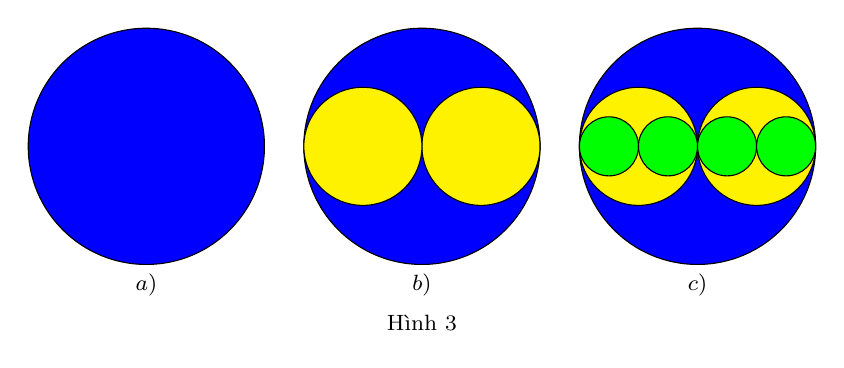
\begin{tikzpicture}[>=stealth,line join=round,line cap=round,font=\footnotesize,scale=1,declare function={r=1.5;}]
			\begin{scope}
				\draw[fill=blue] (0,0)circle(r);
				\path (0,-r) node[below]{$a)$};
			\end{scope}
			\begin{scope}[xshift={3.5cm}]
				\draw[fill=blue] (0,0)circle(r);
				\draw[fill=yellow] (r/2,0)circle(r/2);
				\draw[fill=yellow] (-r/2,0)circle(r/2);
				\path (0,-r) node[below]{$b)$};
			\end{scope}
			\begin{scope}[xshift={7cm}]
				\draw[fill=blue] (0,0)circle(r);
				\draw[fill=yellow] (r/2,0)circle(r/2);
				\draw[fill=yellow] (-r/2,0)circle(r/2);
				\foreach \i in {0,1,2,3}
				\draw[fill=green,shift={(r/2*\i,0)}] (-3*r/4,0)circle(r/4);
				\path (0,-r) node[below]{$c)$};
			\end{scope}
			\path (current bounding box.south) node[below]{Hình $3$};
		\end{tikzpicture}
	}
	\loigiai{
		Diện tích của các hình tròn trong các lần cắt là
		\begin{enumerate}
			\item Lần thứ 1: $S_1=\pi R^2$.
			\item  Lần thứ 2: $S_2=2\cdot \pi \left(\dfrac{R}{2}\right)^2= \dfrac{\pi R^2}{2}$.
			\item  Lần thứ 3: $S_2=4\cdot \pi \left(\dfrac{R}{4}\right)^2= \dfrac{\pi R^2}{2^2}$.	
			\item Lần thứ $n$: $S_n= \dfrac{\pi R^2}{2^{n-1}}$.
		\end{enumerate}
		Do đó  diện tích các hình tròn lập thành một cấp số nhân lùi vô hạn có số hạng đầu $S_1=\pi R^2$ và công bội $q=\dfrac{1}{2}$ nên tổng diện tích các hình tròn là 
		\[ S_1+S_2+\cdots=\dfrac{\pi R^2}{1-\dfrac{1}{2}}=2\pi R^2. \]
	}
\end{bt}
\begin{bt}%[1T3K1-5]
	\immini{
		Từ hình vuông đầu tiên có cạnh bằng $1$ (đơn vị độ dài), nối các trung điểm của bốn cạnh để có hình vuông thứ hai. Tiếp tục nối các trung điểm của bốn cạnh của hình vuông thứ hai để được hình vuông thứ ba. Cứ tiếp tục làm như thế, nhận được một dãy hình vuông (xem Hình $5$).
	}{\hspace*{.5cm}
		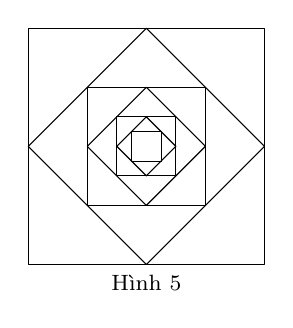
\begin{tikzpicture}[>=stealth,line join=round,line cap=round,font=\footnotesize,scale=1,declare function={a=3;}]
			\foreach \i in {1,2,...,7}{
				\pgfmathsetmacro\r{a*(sin(45))^(\i-1)}
				\pgfmathsetmacro{\j}{int(mod(\i,2))}
				\ifnum \j=1
				\draw (-\r/2,-\r/2) rectangle (\r/2,\r/2);
				\else
				\draw[rotate=45] (-\r/2,-\r/2) rectangle (\r/2,\r/2);
				\fi
			}
			\path (current bounding box.south) node[below]{Hình $5$};
		\end{tikzpicture}\hspace*{1cm}
	}
	\begin{enumerate}
		\item Kí hiệu $a_n$ là diện tích của hình vuông thứ $n$ và $S_n$ là tổng diện tích của $n$ hình vuông đầu tiên. Viết công thức tính $a_n$, $S_n$ ($n=1,2,3, \ldots$) và tìm $\lim \limits_{n \to +\infty}S_n$ (giới hạn này nếu có được gọi là tổng diện tích của các hình vuông).
		\item Kí hiệu $p_n$ là chu vi của hình vuông thứ $n$ và $Q_n$ là tổng chu vi của $n$ hình vuông đầu tiên. Viết công thức tính $p_n$ và $Q_n$ $(n=1,2,3, \ldots)$ và tìm $\lim \limits_{n \to +\infty}Q_n$ (giới hạn này nếu có được gọi là tổng chu vi của các hình vuông).
	\end{enumerate}
	\loigiai{
		\begin{enumerate}
			\item Ta có hình vuông thứ nhất có cạnh bằng $1$,
			hình vuông thứ hai có cạnh bằng $\dfrac{\sqrt{2}}{2}$.\\
			Hình vuông thứ ba có cạnh bằng $\dfrac{1}{2}$.\\
			Suy ra	hình vuông thứ $n$ có cạnh bằng $\left(\dfrac{\sqrt{2}}{2}\right)^{n-1}$.\\
			Diện tích của hình vuông thứ $n$ là $a_n=\left(\dfrac{\sqrt{2}}{2}\right)^{n-1}\cdot \left(\dfrac{\sqrt{2}}{2}\right)^{n-1}=\left(\dfrac{1}{2}\right)^{n-1}$.\\
			Tổng diện tích của $n$ hình vuông đầu tiên là tổng của cấp số nhân có  số hạng đầu $a_1=1$ và công bội $q=\dfrac{1}{2}$ nên
			\[ S_n=\dfrac{a_1\left(1-q^n\right)}{1-q}=\dfrac{1-\left(\dfrac{1}{2}\right)^n}{1-\dfrac{1}{2}}=2\left[1-\left(\dfrac{1}{2}\right)^n\right].\]
			$\lim \limits_{n \to +\infty}S_n=\lim \limits_{n \to +\infty}2\left[1-\left(\dfrac{1}{2}\right)^n\right]=2 \left[\lim \limits_{n \to +\infty}1-\lim \limits_{n \to +\infty}\left(\dfrac{1}{2}\right)^n\right]=2 $.
			\item Hình vuông thứ nhất có chu vi bằng $4$, hình vuông thứ $2$ có chu vi là $2\sqrt{2}$, hình vuông thứ $3$ có chu vi là $2$.\\
			Suy ra hình vuông thứ $n$ có chu vi bằng $p_n=4\cdot \left(\dfrac{\sqrt{2}}{2}\right)^{n-1}$.
			Tổng chu vi của $n$ hình vuông đầu tiên là tổng của cấp số nhân có  số hạng đầu $p_1=4$ và công bội $q=\dfrac{\sqrt{2}}{2}$ nên 
			\[ Q_n=\dfrac{p_1\left(1-q^n\right)}{1-q}=\dfrac{4\left(1-\left(\dfrac{\sqrt{2}}{2}\right)^n\right)}{1-\dfrac{\sqrt{2}}{2}}=\left(8+4\sqrt{2}\right)\left[1-\left(\dfrac{\sqrt{2}}{2}\right)^n\right].\]
			$\lim \limits_{n \to +\infty}Q_n=\left(8+4\sqrt{2}\right)\lim \limits_{n \to +\infty}\left[1-\left(\dfrac{\sqrt{2}}{2}\right)^n\right]=\left(8+4\sqrt{2}\right)\left(1-0\right)=8+4\sqrt{2}$.
		\end{enumerate}	
	}
\end{bt}

\begin{bt}%[1T3K1-4]
	Xét quá trình tạo ra hình có chu vi vô cực và diện tích bằng $0$ như sau:\\ Bắt đầu bằng một hình vuông $H_0$ cạnh bằng 1 đơn vị độ dài (xem Hình $6a$). Chia hình vuông $H_0$ thành chín hình vuông bằng nhau, bỏ đi bốn hình vuông, nhận được hình $H_1$ (xem Hình $6b$). Tiếp theo, chia mỗi hình vuông của $H_1$ thành chín hình vuông, rồi bỏ đi bốn hình vuông, nhận được hình $H_2$ (xem Hình $6c$). Tiếp tục quá trình này, ta nhận được một dãy hình $H_n$ $(n=1,2,3,\ldots)$.	
	\\[1mm]
	\centerline{
		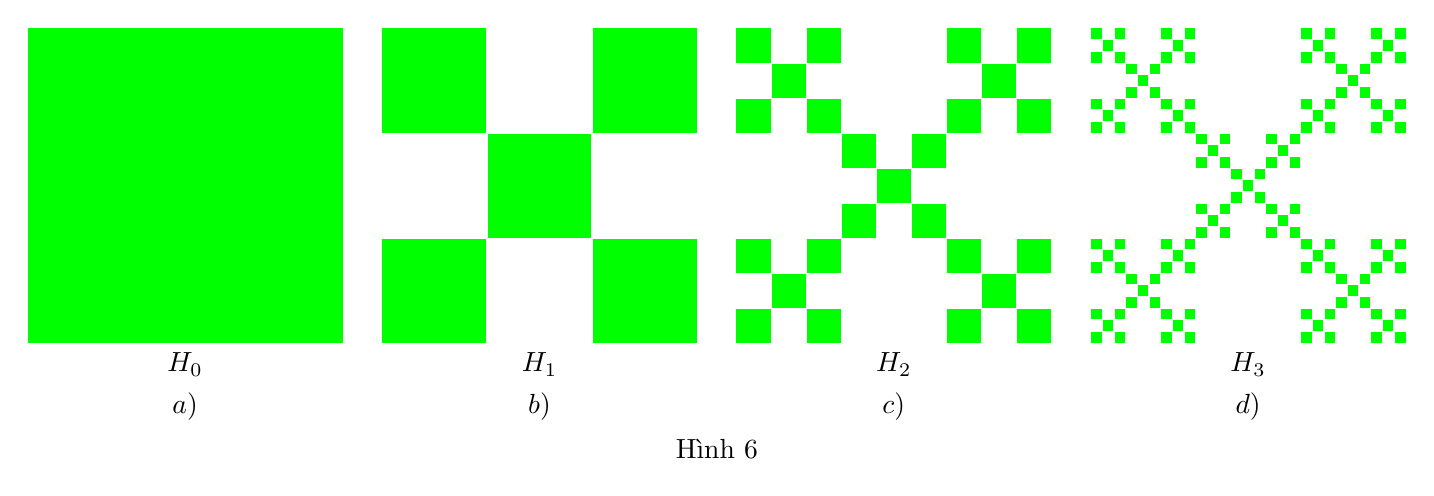
\begin{tikzpicture}% Muốn vẽ hình Hn thì dùng \hv{n}
			\def\a{2}
			\pgfmathsetmacro\sh{2*\a *sqrt(2)/3}
			\def\hv#1{
				\ifnum#1>0
				\draw[white,fill=white] 
				(-\a/3,\a/3) rectangle (\a/3,\a)
				(-\a/3,-\a/3) rectangle (-\a,\a/3)
				(-\a/3,-\a/3) rectangle (\a/3,-\a)
				(\a/3,-\a/3) rectangle (\a,\a/3)
				;
				\pgfmathtruncatemacro{\k}{#1-1}
				\begin{scope}[scale=1/3]\hv{\k}\end{scope}
				\begin{scope}[shift={(45:\sh)},scale=1/3]\hv{\k}\end{scope}
				\begin{scope}[shift={(135:\sh)},scale=1/3]\hv{\k}\end{scope}
				\begin{scope}[shift={(225:\sh)},scale=1/3]\hv{\k}\end{scope}
				\begin{scope}[shift={(315:\sh)},scale=1/3]\hv{\k}\end{scope}
				\fi
			}
			\begin{scope}
				\fill[green] (-\a,-\a) rectangle (\a,\a);
				\hv{0}
				\path (0,-\a)node[below]{$H_0$}
				node[below=.5cm]{$a)$};
			\end{scope}
			\begin{scope}[xshift=4.5cm]
				\fill[green] (-\a,-\a) rectangle (\a,\a);
				\hv{1}
				\path (0,-\a)node[below]{$H_1$}
				node[below=.5cm]{$b)$};
			\end{scope}
			\begin{scope}[xshift=9cm]
				\fill[green] (-\a,-\a) rectangle (\a,\a);
				\hv{2}
				\path (0,-\a)node[below]{$H_2$}
				node[below=.5cm]{$c)$};
			\end{scope}
			\begin{scope}[xshift=13.5cm]
				\fill[green] (-\a,-\a) rectangle (\a,\a);
				\hv{3}
				\path (0,-\a)node[below]{$H_3$}
				node[below=.5cm]{$d)$};
			\end{scope}
			\path (current bounding box.south) node[below]{Hình $6$};
		\end{tikzpicture}
	}
	Ta có: $H_1$ có $5$ hình vuông, mỗi hình vuông có cạnh bằng $\dfrac{1}{3}$;\\
	{\color{white}{Ta có: }}$H_2$ có $5\cdot5=5^2$ hình vuông, mỗi hình vuông có cạnh bằng $\dfrac{1}{3} \cdot \dfrac{1}{3}=\dfrac{1}{3^2}; \ldots$.\\
	Từ đó, nhận được $H_n$ có $5^n$ hình vuông, mỗi hình vuông có cạnh bằng $\dfrac{1}{3^n}$.
	\begin{enumerate}
		\item Tính diện tích $S_n$ của $H_n$ và tính $\lim \limits_{n \to +\infty}S_n$.
		\item Tính chu vi $p_n$ của $H_n$ và tính $\lim \limits_{n \to +\infty}p_n$.
	\end{enumerate}
	(Quá trình trên tạo nên một hình, gọi là một fractal, được coi là có diện tích $\lim \limits_{n \to +\infty}S_n$ và chu vi $\lim \limits_{n \to +\infty}p_n$).
	\loigiai{
		\begin{enumerate}
			\item Hình vuông $H_1$ có diện tích $S_1=5\cdot \left(\dfrac{1}{3}\right)^2=\dfrac{5}{9}$.\\
			Hình vuông $H_2$ có diện tích $S_2=5^2\cdot \left(\dfrac{1}{3^2}\right)^2=\left(\dfrac{5}{9}\right)^2$.\\
			Hình vuông $H_n$ có diện tích $S_n=5^n\cdot \left(\dfrac{1}{3^n}\right)^2=\left(\dfrac{5}{9}\right)^n$.\\
			$\lim \limits_{n \to +\infty}S_n=\lim \limits_{n \to +\infty}\left(\dfrac{5}{9}\right)^n=0$.
			\item Hình vuông $H_1$ có chu vi $p_1=5\cdot 4\cdot  \dfrac{1}{3}=4\cdot \dfrac{5}{3}$.\\
			Hình vuông $H_2$ có chu vi $p_2=5^2\cdot4\cdot \dfrac{1}{3^2}=4\cdot \left(\dfrac{5}{3}\right)^2$.\\
			Hình vuông $H_n$ có diện tích $p_n=5^n\cdot4\cdot  \dfrac{1}{3^n}=4\cdot \left(\dfrac{5}{3}\right)^n$.\\
			$\lim \limits_{n \to +\infty}p_n=\lim \limits_{n \to +\infty}4\cdot \left(\dfrac{5}{3}\right)^n=+\infty$.
		\end{enumerate}
	}
\end{bt}
\begin{bt}%[1T3K1-5]
	\immini{Cho tam giác đều có cạnh bằng $a$, gọi là tam giác $H_1$. Nối các trung điểm của $H_1$ để tạo thành tam giác $\mathrm{H}_2$. Tiếp theo, nối các trung điểm của $\mathrm{H}_2$ để tạo thành tam giác $\mathrm{H}_3$ (Hình bên). Cứ tiếp tục như vậy, nhận được dãy tam giác $H_1, H_2, H_3, \ldots$\\
		Tính tổng chu vi và tổng diện tích các tam giác của dãy.}{
		\begin{tikzpicture}[scale=1, font=\footnotesize, line join=round, line cap=round, >=stealth]
			(0,0) coordinate (A)	
			(4,0) coordinate (B)	
			(2,2.8284) coordinate (C)
			\draw (A)--(B)--(C)--cycle;
			\coordinate (I) at ($(A)!0.5!(B)$);
			\coordinate (J) at ($(B)!0.5!(C)$);
			\coordinate (K) at ($(C)!0.5!(A)$);
			\draw (I)--(J)--(K)--cycle;
			\coordinate (H) at ($(I)!0.5!(J)$);
			\coordinate (G) at ($(J)!0.5!(K)$);
			\coordinate (F) at ($(K)!0.5!(I)$);
			\draw (H)--(G)--(F)--cycle;
			\coordinate (X) at ($(H)!0.5!(G)$);
			\coordinate (Y) at ($(G)!0.5!(F)$);
			\coordinate (Z) at ($(F)!0.5!(H)$);
			\draw (X)--(Y)--(Z)--cycle;
			\draw[dashed] (2,2.8284)--(3.3,1.45)node[above right]{$a$}--(4,0);
		\end{tikzpicture}
	}
	\loigiai{
		Gọi $S_i$ và $C_i$ ($i=1,2,\ldots$) lần lượt là diện tích và chu vi của tam giác $H_i$, $i=1,2,\ldots $.\\
		Khi đó ta có
		\begin{itemize}
			\item[$\bullet$] $S_1=\dfrac{a^2\sqrt{3}}{4};S_2=\left(\dfrac{a}{2}\right)^2\dfrac{\sqrt{3}}{4}=\dfrac{a^2\sqrt{3}}{16}=\dfrac{S_1}{4};S_3=\dfrac{1}{4}S_2,\ldots $.\\
			Do đó $(S_n)$ là một cấp số nhân lùi vô hạn với $S_1=\dfrac{a^2\sqrt{3}}{4}$ và $q_1=\dfrac{1}{4}$.\\
			Tổng diện tích $S=S_1+S_2+\cdots =\dfrac{S_1}{1-q_1}=\dfrac{a^2\sqrt{3}}{3}$.
			\item[$\bullet$] $C_1=3a; C_2=\dfrac{3a}{2}=\dfrac{1}{2}C_1,\ldots$\\
			Do đó $(C_n)$ là một cấp số nhân lùi vô hạn với $C_1=3a;q_2=\dfrac{1}{2}$.\\
			Tổng chu vi là $C=C_1+C_2+\cdots =\dfrac{C_1}{1-q_2}=6a$.
		\end{itemize}
	}	
\end{bt}
\begin{bt}%[1D4K1-6]
	Một thấu kính hội tụ có tiêu cự là $f$. Gọi $d$ và $d^{\prime}$ lần lượt là khoảng cách từ một vật thật $A B$ và từ ảnh $A^{\prime} B^{\prime}$ của nó tới quang tâm $O$ của thấu kính như hình vẽ bên dưới. Công thức thấu kính là $\dfrac{1}{d}+\dfrac{1}{d}=\dfrac{1}{f}$.
	\begin{center}
		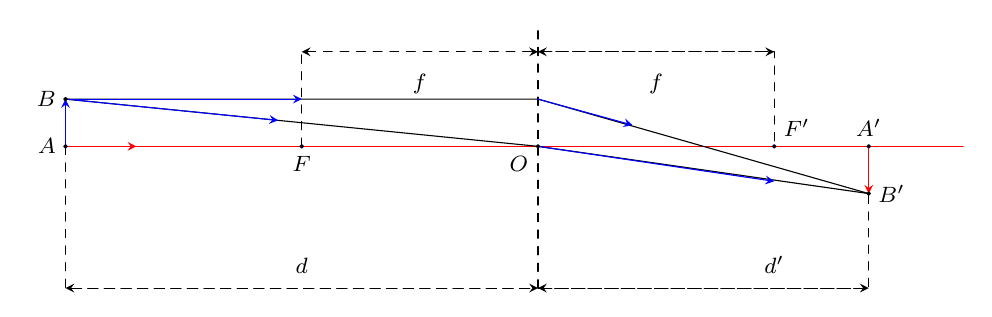
\begin{tikzpicture}[scale=0.6, font=\footnotesize, line join=round, line cap=round, >=stealth]		
			%\draw[domain=-3.65:3.65, blue,] plot({3/10*(\x)^2},\x);
			%\draw[gray!10] (-1,-1) grid (5,5);
			\draw [red] (-10,0)--(9,0);
			\draw [dashed] (0,-3)--(0,2.5);
			\coordinate (A) at (-10,0); 
			\coordinate (A') at (7,0); 
			\coordinate (B) at (-10,1); 
			\coordinate (L) at ( 0,1);
			\coordinate (O) at (0,0); 
			\coordinate (B') at (7,-1); 
			\coordinate (F') at (5,0); 
			\coordinate (F) at (-5,0); 
			\coordinate (H) at (-5,1); 
			\coordinate (M) at (5,2); 
			\coordinate (M') at (-5,2); 
			\coordinate (S) at (-10,-3); 
			\coordinate (K) at (7,-3);
			\coordinate (K') at (-5.5,0.55); 
			\coordinate (N) at (5,-0.74); 
			\coordinate (G) at (2,0.45); 
			\coordinate (Q) at (-2.5,0.9); 
			\coordinate (Q') at (2.5,0.9);
			\coordinate (J) at (-5,-2.9); 
			\coordinate (J') at (5,-2.9);
			\coordinate (X) at (-8.5,0);
			\coordinate (V) at (0,-3); \coordinate (V') at (0,2);
			%\draw  (F)--(D) (G)--(C) (F')--(D') (G')--(C') ;
			\draw (B)--(L)--(B');
			\draw (B)--(O)--(B');\draw[red,->] (A)--(X);
			\draw[blue,->] (B)--(H); \draw[blue,->] (B)--(K');
			\draw[blue,->] (A)--(B); \draw[blue,->] (O)--(N);
			\draw[blue,->] (L)--(G); \draw[red,->] (A')--(B');
			\draw[dashed] (F)--(M')--(M)--(F');
			\draw[dashed] (A)--(S)--(K)--(B');
			\draw[dashed,<->] (S)--(V);\draw[dashed,<->] (V)--(K) ;
			\draw[dashed,<->] (M')--(V');\draw[dashed,<->] (V')--(M) ;
			%\draw[red,->] (E)--(H3); 
			%\draw[->] (C)--(K3) ;
			%\draw[red,->] (E)--(H4); 
			%\draw[->] (C')--(K4) ;
			%\draw[red,->] (E)--(H2); 
			%\draw[->] (D')--(K2) ;
			
			%\draw[red] (E)--(C) (E)--(D) (E)--(C') (E)--(D');
			\draw[fill=black] (A') circle (1pt) node [above] {$A'$};
			\draw (Q) node [above] {$f$}; \draw (Q') node [above] {$f$}; \draw (J) node [above] {$d$}; \draw (J') node [above] {$d'$};
			\draw[fill=black] (B') circle (1pt) node [right] {$B'$};
			\draw[fill=black] (F') circle (1pt) node [above right] {$F'$};
			\draw[fill=black] (F) circle (1pt) node [below] {$F$};
			\draw[fill=black] (A) circle (1pt) node [left] {$A$};
			\draw[fill=black] (B) circle (1pt) node [left] {$B$};
			%\draw[fill=black] (E) circle (1pt) node [below right] {$S$};
			\draw[fill=black] (O) circle (1pt) node [below left] {$O$};
		\end{tikzpicture}
	\end{center}
	\begin{listEX}
		\item[a)] Tìm biểu thức xác định hàm số $d^{\prime}=\varphi(d)$.
		\item[b)] Tìm $\underset{d \rightarrow f^{+}}\lim \limits_{n \to +\infty}\varphi(d), \underset{d \rightarrow f^{-}}\lim \limits_{n \to +\infty}\varphi(d)$ và $\underset{d \rightarrow f}\lim \limits_{n \to +\infty}\varphi(d)$. Giải thích ý nghĩa của các kết quả tìm được.
	\end{listEX}
	\loigiai{
		\begin{listEX}
			\item[a)] Ta có $$\dfrac{1}{d}+\dfrac{1}{d^{\prime}}=\dfrac{1}{f} \Leftrightarrow d^{\prime}=\dfrac{d f}{d-f}.$$
			Vậy $\varphi(d)=\dfrac{d f}{d-f}$.		
			\item[b)] Vì $\underset{d \rightarrow f^{+}}\lim \limits_{n \to +\infty}df=f^2; \underset{d \rightarrow f^{+}}\lim \limits_{n \to +\infty}(d-f)=0 ; d \rightarrow f^{+} \Rightarrow d-f>0 $ nên $ \underset{d \rightarrow f^{+}}\lim \limits_{n \to +\infty} \dfrac{d f}{d-f}=+\infty$.\\
			Vậy $\underset{d \rightarrow f^{+}}\lim \limits_{n \to +\infty}\varphi(d)=\underset{d \rightarrow f^{+}}\lim \limits_{n \to +\infty} \dfrac{d f}{d-f}=+\infty$.\\
			\textbf{Ý nghĩa}: Khi đặt vật nằm ngoài tiêu cự và tiến dần đến tiêu điểm thì cho ảnh thật ngược chiều với vật ở vô cùng.\\
			Vì $\underset{d \rightarrow f^{-}}\lim \limits_{n \to +\infty}df=f^2; \underset{d \rightarrow f^{+}}\lim \limits_{n \to +\infty}(d-f)=0 ; d \rightarrow f^{-} \Rightarrow d-f<0 $ nên $ \underset{d \rightarrow f^{+}}\lim \limits_{n \to +\infty} \dfrac{d f}{d-f}=-\infty$.\\
			Vậy $\underset{d \rightarrow f^{+}}\lim \limits_{n \to +\infty}\varphi(d)=\underset{d \rightarrow f^{+}}\lim \limits_{n \to +\infty} \dfrac{d f}{d-f}=-\infty$.\\
			\textbf{Ý nghĩa}: Khi đặt vật nằm trong tiêu cự và tiến dần đến tiêu điểm thì cho ảnh ảo cùng chiều với vật và nằm ở vô cùng.\\
			Vì không tồn tại $\underset{d \rightarrow f^{+}}\lim \limits_{n \to +\infty}\varphi(d)$ và $\underset{d \rightarrow f^{-}}\lim \limits_{n \to +\infty}\varphi(d)$ nên không tồn tại $\underset{d \rightarrow f}\lim \limits_{n \to +\infty}\varphi(d)$.
		\end{listEX}
	}
\end{bt}
\subsection*{Bài tập trắc nghiệm}
\Opensolutionfile{ans}[ans/ans-1K1-5-csn-lui]
\begin{ex}%[1C3K1-6]
	Có $1$ kg chất phóng xạ độc hại. Biết rằng, cứ sau một khoảng thời gian $T=24000$ năm thì một nửa số chất phóng xạ này bị phân rã thành chất khác không độc hại đối với sức khỏe của con người ($T$ được gọi là \textit{chu kì bán rã}). Gọi $u_n$ là khối lượng chất phóng xạ còn lại sau chu kì thứ $n$.
	Sau ít nhất bao nhiêu chu kì bán rã thì khối lượng phóng xạ đã cho ban đầu không còn độc hại với con người, biết rằng chất phóng xạ này sẽ không độc hại nữa nếu khối lượng chất phóng xạ còn lại bé hơn $10^{-6}$ g.
	\choice
	{$24$}
	{\True $30$}
	{$100$}
	{$15$}
	\loigiai{
		\item Chất phóng xạ sẽ không độc hại nữa nếu khối lượng chất phóng xạ còn lại bé hơn $10^{-6}~\mathrm{g}=10^{-9}$ kg
		$$\Leftrightarrow u_n<10^{-9}\Leftrightarrow\dfrac{1}{2^n}<10^{-9}\Leftrightarrow 2^n>10^9\Leftrightarrow n\geq 30.$$
		Vậy sau ít nhất $30$ chu kì thì khối lượng phóng xạ đã cho ban đầu không còn độc hại với con người nữa.
	}
\end{ex}
\begin{ex}%[1C3K1-6]
	Có $1$ kg chất phóng xạ độc hại. Biết rằng, cứ sau một khoảng thời gian $T=24000$ năm thì một nửa số chất phóng xạ này bị phân rã thành chất khác không độc hại đối với sức khỏe của con người ($T$ được gọi là \textit{chu kì bán rã}). Gọi $u_n$ là khối lượng chất phóng xạ còn lại sau chu kì thứ $n$.
	Sau ít nhất bao nhiêu năm thì khối lượng phóng xạ đã cho ban đầu không còn độc hại với con người, biết rằng chất phóng xạ này sẽ không độc hại nữa nếu khối lượng chất phóng xạ còn lại bé hơn $10^{-6}$ g.
	\choice
	{$30$}
	{$2400$}
	{\True $720000$}
	{$10000$}
	\loigiai{
		\item Chất phóng xạ sẽ không độc hại nữa nếu khối lượng chất phóng xạ còn lại bé hơn $10^{-6}~\mathrm{g}=10^{-9}$ kg
		$$\Leftrightarrow u_n<10^{-9}\Leftrightarrow\dfrac{1}{2^n}<10^{-9}\Leftrightarrow 2^n>10^9\Leftrightarrow n\geq 30.$$
		Vậy sau ít nhất $30$ chu kì bằng $30\cdot 24000=720000$ năm thì khối lượng phóng xạ đã cho ban đầu không còn độc hại với con người nữa.
	}
\end{ex}
\begin{ex}%[1C3K1-6]
	Từ hình vuông có độ dài cạnh bằng $1$, người ta nối các trung điểm của cạnh hình vuông để tạo ra hình vuông mới như hình bên. Tiếp tục quá trình này đến vô hạn. Tính tổng diện tích của tất cả các hình vuông được tạo thành.
	\choice
	{$1$}
	{\True $2$}
	{$3$}
	{$4$}	
	\loigiai{
		Từ giả thiết suy ra diện tích hình vuông sau bằng $\dfrac{1}{2}$ diện tích hình vuông trước.\\ 
		Khi đó diện tích của các hình vuông tạo thành một cấp số nhân lùi vô hạn với số hạng đầu $S_1=1$ và công bội $q=\dfrac{1}{2}$.\\
		Diện tích $S_n$ của hình vuông được tạo thành từ bước thứ $n$ là $S_n=S_1\cdot q^{n-1}=\left(\dfrac{1}{2}\right)^{n-1}$.\\
		Tổng diện tích của tất cả các hình vuông được tạo thành là:\\
		$$S=\dfrac{u_1}{1-q}=\dfrac{1}{1-\dfrac{1}{2}}=2.$$		
	}
\end{ex}
\begin{ex}%[1T3K1-5]
	Từ hình vuông đầu tiên có cạnh bằng $1$ (đơn vị độ dài), nối các trung điểm của bốn cạnh để có hình vuông thứ hai. Tiếp tục nối các trung điểm của bốn cạnh của hình vuông thứ hai để được hình vuông thứ ba. Cứ tiếp tục làm như thế, nhận được một dãy hình vuông. Tính tổng chu vi của dãy các hình vuông trên. 
	\choice
	{$8+\sqrt{2}$}
	{$2+\sqrt{2}$}
	{\True $8+4\sqrt{2}$}
	{$4+4\sqrt{2}$}
	\loigiai{
		Hình vuông thứ nhất có chu vi bằng $4$, hình vuông thứ $2$ có chu vi là $2\sqrt{2}$, hình vuông thứ $3$ có chu vi là $2$.\\
		Suy ra hình vuông thứ $n$ có chu vi bằng $p_n=4\cdot \left(\dfrac{\sqrt{2}}{2}\right)^{n-1}$.
		Tổng chu vi của $n$ hình vuông đầu tiên là tổng của cấp số nhân có  số hạng đầu $p_1=4$ và công bội $q=\dfrac{\sqrt{2}}{2}$ nên 
		\[ Q_n=\dfrac{p_1\left(1-q^n\right)}{1-q}=\dfrac{4\left(1-\left(\dfrac{\sqrt{2}}{2}\right)^n\right)}{1-\dfrac{\sqrt{2}}{2}}=\left(8+4\sqrt{2}\right)\left[1-\left(\dfrac{\sqrt{2}}{2}\right)^n\right].\]
		$\lim \limits_{n \to +\infty}Q_n=\left(8+4\sqrt{2}\right)\lim \limits_{n \to +\infty}\left[1-\left(\dfrac{\sqrt{2}}{2}\right)^n\right]=\left(8+4\sqrt{2}\right)\left(1-0\right)=8+4\sqrt{2}$.
	}
\end{ex}
\begin{ex}%[1D4K1-6]
	Từ độ cao $55,8 \mathrm{~m}$ của tháp nghiêng Pisa nước Ý, người ta thả một quả bóng cao su chạm xuống đất hình bên dưới. Giả sử mỗi lần chạm đất quả bóng lại nảy lên độ cao bằng $\dfrac{1}{10}$ độ cao mà quả bóng đạt được trước đó. Gọi $S_n$ là tổng độ dài quãng đường di chuyển của quả bóng tính từ lúc thả ban đầu cho đến khi quả bóng đó chạm đất $n$ lần. Tính $\lim \limits_{n \to +\infty}S_n$.
	\choice
	{$58{,}8$}
	{$67{,}2$}
	{$68$}
	{\True $68{,}2$}
	\loigiai{Mỗi khi chạm đất quả bóng lại nảy lên một độ cao bằng $\dfrac{1}{10}$ độ cao của lần rơi ngay trước đó và sau đó lại rơi xuống từ độ cao thứ hai này. Do đó, độ dài hành trình của quả bóng kể từ thời điểm rơi ban đầu đến:\\    
		Thời điểm chạm đất lần thứ nhất là $d_1=55{,}8$.\\
		Thời điềm chạm đất lần thứ hai là $d_2=55{,}8+2\cdot \dfrac{55{,}8}{10}$.\\
		Thời điểm chạm đất lần thứ ba là $d_3=55{,}8+2 \cdot\dfrac{55{,}8}{10}+2\cdot \dfrac{55{,}8}{10^2}$.\\
		Thời điểm chạm đất lần thứ tư là $d_4=55{,}8+2 \cdot\dfrac{55{,}8}{10}+2\cdot \dfrac{55,8}{10^2}+2\cdot \dfrac{55{,}8}{10^3}$.\\
		$\ldots$\\
		Thời điểm chạm đất lần thứ $n~(n>1)$ là
		$$d_n=55{,}8+2\cdot55{,}8+2\cdot \frac{55{,}8}{10^2}+2\cdot \frac{55{,}8}{10^3}+\ldots+2\cdot \frac{55{,}8}{10^{n-1}}.$$
		Do đó, quãng đường mà quả bóng đi được kể từ thời điềm rơi đến khi nằm yên trên mặt đất là:
		$$ d=55{,}8+2.55{,}8+2\cdot \frac{55{,}8}{10^2}+2\cdot \frac{55{,}8}{10^3}+\ldots+2\cdot \frac{55{,}8}{10^{n-1}}+\ldots=\lim \limits_{n \to +\infty}d_n.$$
		Vì $2\cdot \dfrac{55{,}8}{10} ; 2\cdot \dfrac{55{,}8}{10^2} ; 2\cdot \dfrac{55{,}8}{10^3}; \ldots ; 2\cdot \dfrac{55{,}8}{10^{n-1}}; \ldots$ là một cấp số nhân lùi vô hạn với công bội $q=\dfrac{1}{10}$ nên ta có:
		$$ 2 \cdot\dfrac{55,8}{10}+2\cdot \dfrac{55{,}8}{10^2}+2\cdot \dfrac{55{,}8}{10^3}+\ldots+2\cdot \dfrac{55{,}8}{10^{n-1}}+\ldots=\dfrac{2\cdot \dfrac{55{,}8}{10}}{1-\dfrac{1}{10}}=12{,}4.$$
		Vậy $d=55{,}8+12{,}4=68{,}2$ m.
	}
\end{ex}
\Closesolutionfile{ans}
\begin{indapan}{10}
	{ans/ans-1K1-5-csn-lui}
\end{indapan}